\documentclass[12pt, fleqn]{article}

\usepackage[utf8]{inputenc}
\usepackage[T2A]{fontenc}
\usepackage{amssymb, amsmath, mathrsfs, amsthm}
\usepackage[russian]{babel}
\usepackage{graphicx}
%\usepackage[footnotesize]{caption3}
\usepackage{indentfirst}
\usepackage[hidelinks]{hyperref}
\usepackage{multirow}
\usepackage{algorithm}
\usepackage{algpseudocode}

% Параметры страницы
\textheight=24cm
\textwidth=16cm
\oddsidemargin=5mm
\evensidemargin=-5mm
\marginparwidth=36pt
\topmargin=-1cm
\footnotesep=3ex
%\flushbottom
\raggedbottom
\tolerance 3000
% подавить эффект "висячих стpок"
\clubpenalty=10000
\widowpenalty=10000

\begin{document}

\begin{titlepage}
\begin{center}
    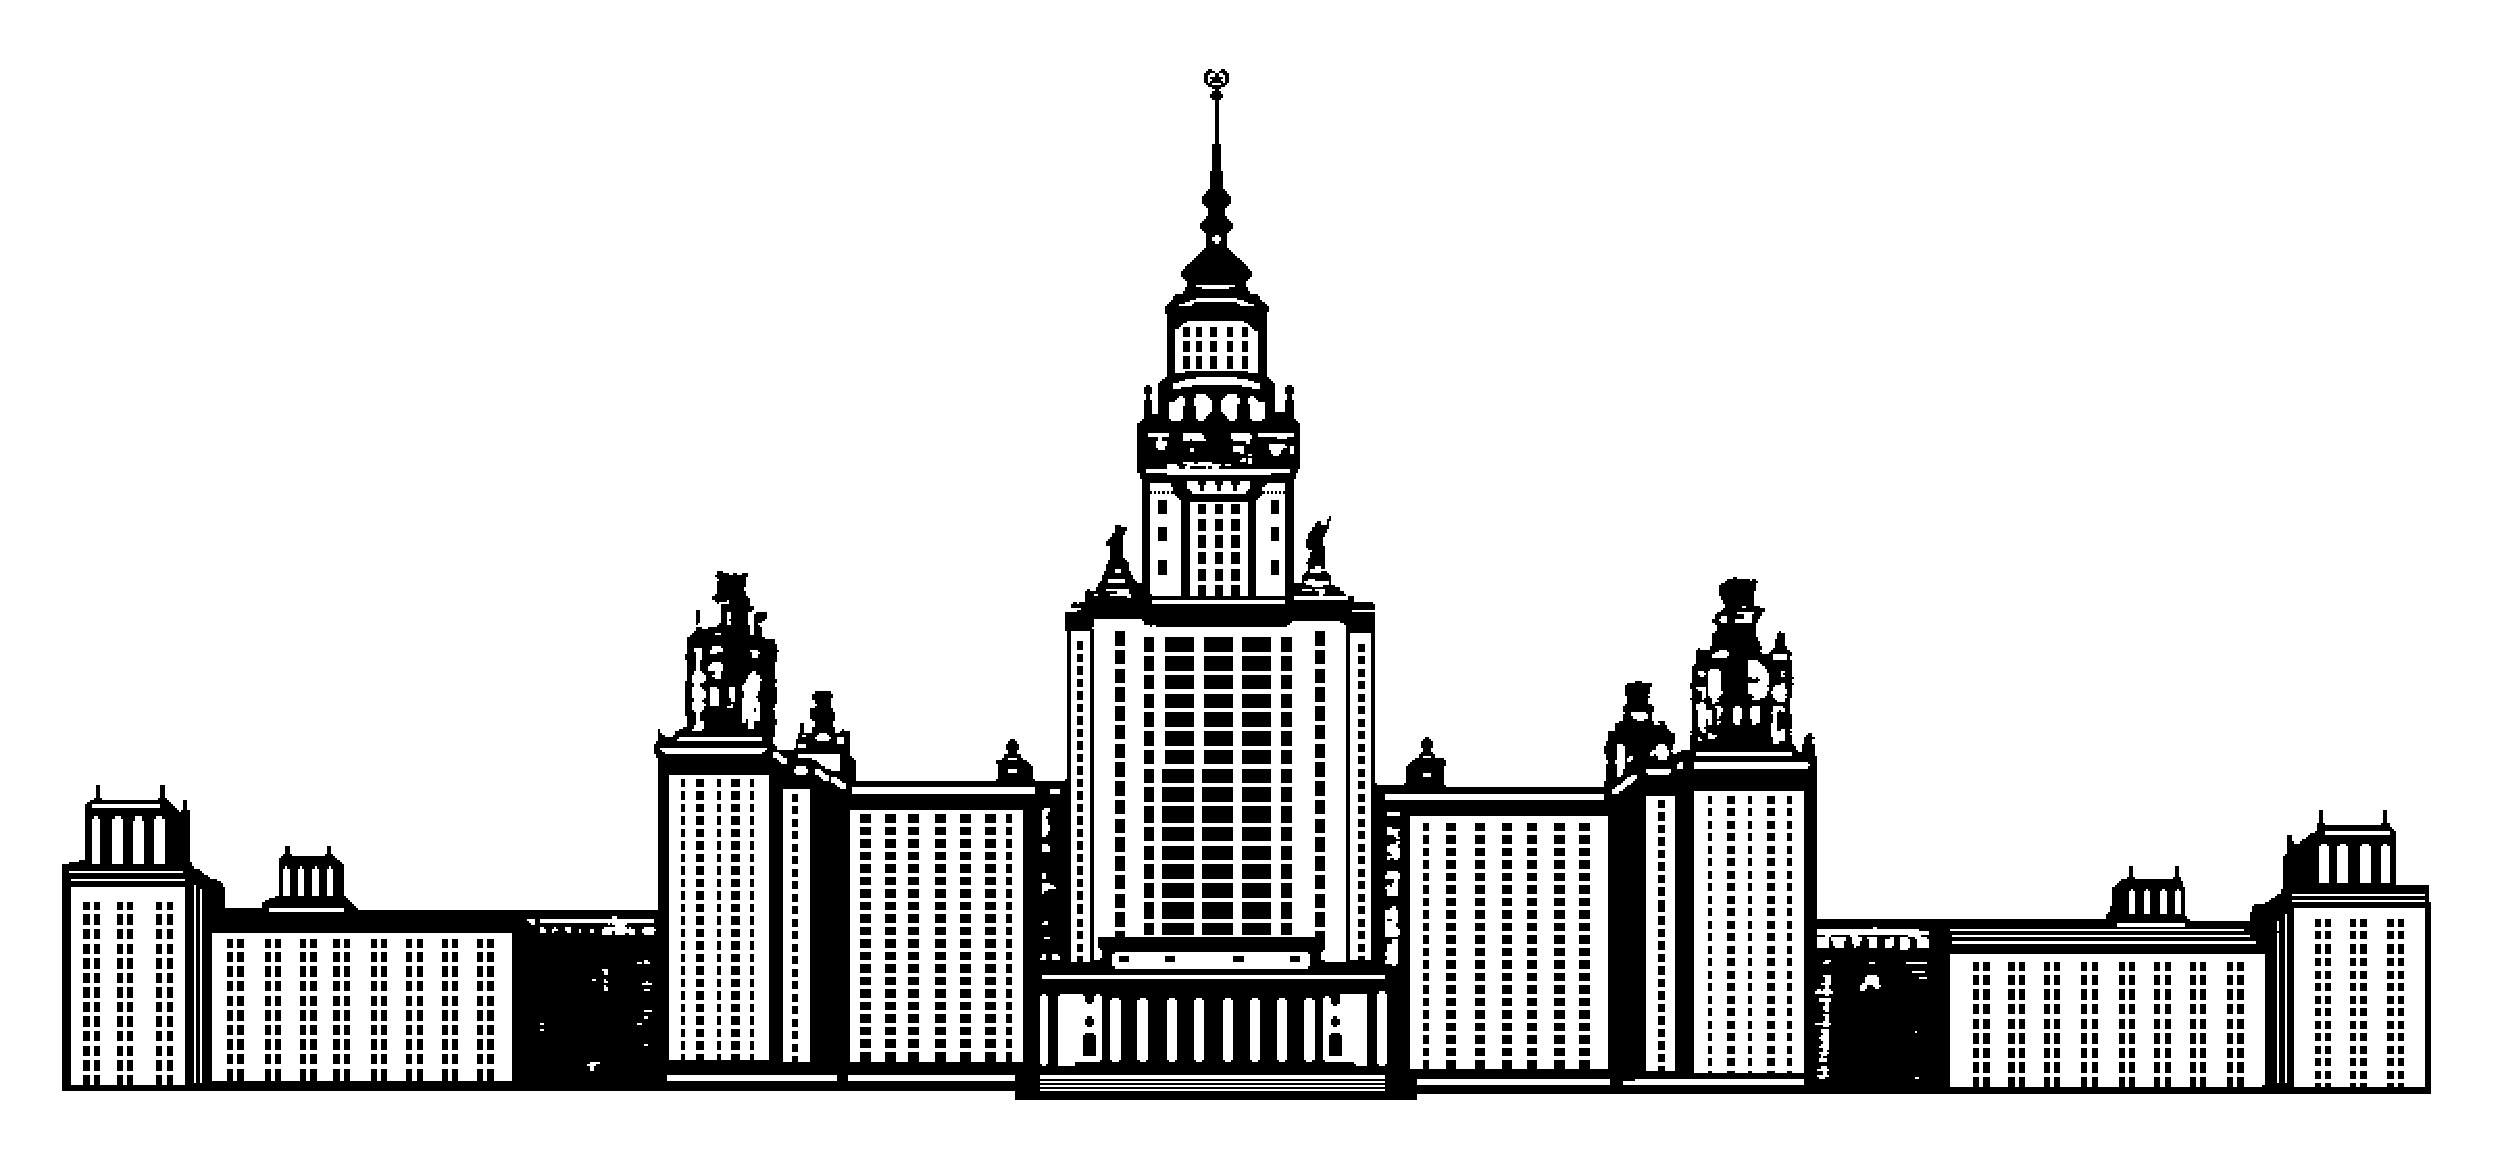
\includegraphics[width=50mm]{msu.eps} \\
    \bigskip
    Московский государственный университет имени М. В. Ломоносова\\
    Факультет Вычислительной Математики и Кибернетики\\
    Кафедра Математических Методов Прогнозирования\\[10mm]

    \textsf{\large
        Лукьянов Павел Александрович\\[15mm]
    }

    \textsf{\Large\bfseries
        Методы аугментации аудиоданных
    }\\[15mm]
    
    \textsf{\Large
        МАГИСТЕРСКАЯ ДИССЕРТАЦИЯ
    }\\[20mm]

    \begin{flushright}
        \parbox{0.5\textwidth}{
            Научный руководитель:\\
            д.ф-м.н., профессор\\
            \emph{Дьяконов Александр Геннадьевич}
        }
    \end{flushright}

    \vspace{\fill}
    Москва, 2022
\end{center}
\end{titlepage}

\newpage
\renewcommand{\contentsname}{Содержание}
\tableofcontents

\newpage

\begin{abstract}
    В данной работе предлагается метод аугментации аудиоданных 
    \newline
    SwapVerticalStripes, основанный на перестановке вертикальных полос в мел-спектрограмме, и его модификации SwapNeighboringStripes, SwapSeveralStripes. Также предлагается алгоритм применения методов аугментации с выбором конкретного метода аугментации после каждой эпохи обучения. Проведенные вычислительные эксперименты показывают возможную применимость предлагаемых подходов в задаче аудиоклассификации.
\end{abstract}

\newpage


\section{Введение}

Понятию аугментации сложно дать точное определение, в данной работе под аугментацией понимается создание новых данных с помощью модификации уже имеющихся. Использование аугментации может быть особенно полезно для небольшой обучающей выборки и может улучшить обобщающую способность модели, являясь мощным инструментом в борьбе с переобучением. 

Исследование методов аугментации данных актуально в настоящее время. Аугментация успешно используется при решении многих задач глубинного обучения, связанных с обработкой изображений, звуковых данных, текстов.

В данной работе рассматриваются методы аугментации аудиоданных, а именно мел-спектрограмм. Мел-спектрограмма получается после применения оконного преобразования Фурье ~\cite{Fourier} и мел-фильтров ~\cite{MelScale}. Мел-спектрограммы представляют собой двумерные матрицы, поэтому их можно рассматривать как изображения и многие подходы к аугментации картинок применимы к аудиоданным. Например, метод Random Erasing ~\cite{RandomErasing}, сводящийся к вырезанию случайных прямоугольников из изображения, может быть использован в задаче аудиоклассификации  ~\cite{RandomErasingClassification}. Также в задаче классификации звуковых данных применяются такие методы аугментации, как Shift Augmentation ~\cite{AudioClassification} --- сдвиг мел-спектрограммы влево или вправо, Noise Augmentation ~\cite{AudioClassification} --- добавление Гауссовского шума, Loudness Augmentation ~\cite{AudioClassification} --- регулирование громкости, Speed augmentation ~\cite{AudioClassification} --- ускорение или замедление аудиозаписи.

SpecAugment ~\cite{SpecAugment} --- один из наиболее известных методов аугментации аудиоданных, который показал свою эффективность в задаче автоматического распознавания речи. Политика аугментации SpecAugment определяется 3 возможными преобразованиями: 
\begin{enumerate}
    \item Time warping ~\cite{SpecAugment} (искривление времени)
    \item Frequency masking ~\cite{SpecAugment} (зануление значений мел-спектрограммы внутри горизонтальной полосы)
    \item Time masking ~\cite{SpecAugment} (зануление значений мел-спектрограммы внутри вертикальной полосы)
\end{enumerate}
В настоящее время известны некоторые модификации SpecAugment: SpliceOut ~\cite{SpliceOut}, SpecAugment++ ~\cite{SpecAugment++}.

В данной работе рассматриваются методы аугментации, которые могут применяться "на лету" (онлайн-аугментация), т.е. преобразования мел-спектрограмм, соответствующие этим аугментациям, должны выполняться достаточно быстро.

На практике выбирается некоторый набор заранее заданных методов аугментации. Пусть $N$ - число выбранных методов ($N \geq 1$). В процессе обучения чаще всего используются следующие стратегии применения методов аугментации:
\begin{enumerate}
    \item к каждому объекту обучающей выборки применяются изначально или во время обучения все $N$ аугментаций. Таким образом, число используемых данных на каждой эпохе увеличивается в $N$ раз.
    \item преобразование, которое будет применено к конкретной мел-спектрограмме, выбирается случайным образом с вероятностью $\frac{1}{N}$ ~\cite{RandAugment}.
\end{enumerate}
Однако возможны и другие стратегии использования методов аугментации. В работе ~\cite{AutoAugment} оптимальная политика применения методов аугментации ищется с помощью методов обучения с подкреплением. В работе ~\cite{MaxUp} предлагается идея минимизации максимальных потерь среди аугментированных данных: \newline
$\min_{\theta} E_{x \sim D} \max_i L(Augment_i(x), \theta)$, где \newline
$D$ --- датасет, \newline
$\theta$ --- параметры нейронной сети, \newline
$L$ --- функция потерь, \newline
$\{Augment_1, Augment_2, ..., Augment_n\}$ --- методы аугментации..

В данной работе предлагается метод аугментации SwapVerticalStripes, основанный на перестановке вертикальных полос в мел-спектрограмме, его модификации SwapNeighboringStripes, SwapSeveralStripes и алгоритм применения методов аугментации с выбором конкретного метода аугментации после каждой эпохи обучения.


\section{Существующие методы аугментации}
Ниже представлены известные подходы к аугментации аудиоданных, используемые в работе. 	
\newline Здесь и далее считаем, что \newline FreqSize --- размерность мел-спектрограммы по частотной оси, \newline TimeSize --- размерность мел-спектрограммы по временной оси, \newline
$S$ --- матрица значений мел-спектрограммы. \newline
Также введем матрицу $M(I, J)$, где $I, J$ --- множества индексов: \newline 
\begin{equation*}
M(I, J) = \{M(i, j)\} = 
\begin{cases}
0, & (i,j) \in I \times J,\\
1, &\text{иначе}.
\end{cases}
\end{equation*}
Стоит рассматривать только случаи, когда в представленных ниже аугментациях значения $t$, $f$, shift ненулевые. В противном случае ($t = 0$, или $f = 0$, или shift = 0) мел-спектрограмма никак не изменяется.

\begin{enumerate}
	\item TimeMasking$^{\ref{fig:i5}}$ ~\cite{SpecAugment} \newline 
	$t \sim U\{0, T\}, t_0 \sim U\{0, \text{TimeSize} - 1 - t\}$, $T$ - параметр аугментации. \newline 
	В результате применения аугментации: \newline
	$S \rightarrow S \cdot M(\{0, \ldots, \text{FreqSize} - 1\}, \{t_0, \ldots, t_0 + t - 1\}) $
	\begin{figure}[ht!]
		\center{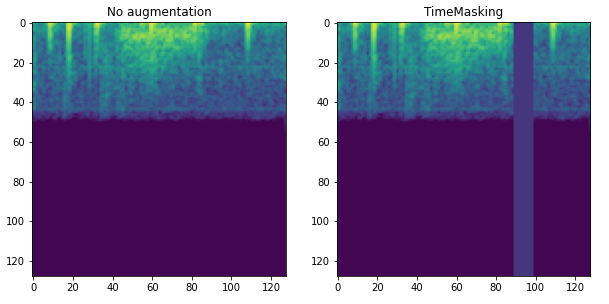
\includegraphics[scale=0.9]{5_0.png}}
		\caption{TimeMasking}
		\label{fig:i5}
	\end{figure}
	\item FreqMasking$^{\ref{fig:i6}}$ ~\cite{SpecAugment} \newline
	$f \sim U\{0, F\}, f_0 \sim U\{0, \text{FreqSize} - 1 - f\}$, $F$ - параметр аугментации. \newline
	В результате применения аугментации: \newline
	$S \rightarrow S \cdot M(\{f_0, \ldots, f_0 + f - 1\}, \{0, \ldots, \text{TimeSize} - 1\}) $
	\begin{figure}[ht!]
		\center{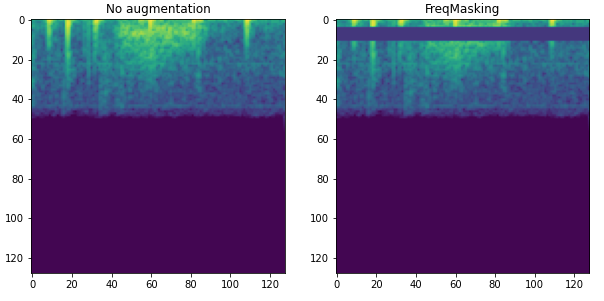
\includegraphics[scale=0.9]{6_0.png}}
		\caption{FreqMasking}
		\label{fig:i6}
	\end{figure}
	\item Noise$^{\ref{fig:i7}}$ ~\cite{AudioClassification}  \newline 
	К каждому значению в мел-спектрограмме добавляется $g \sim N(0, \sigma)$ (для каждого значения мел-спектрограммы генерируется свое g), где $\sigma$ - параметр аугментации (в данной работе $\sigma = 0.01$). 
	\begin{figure}[ht!]
		\center{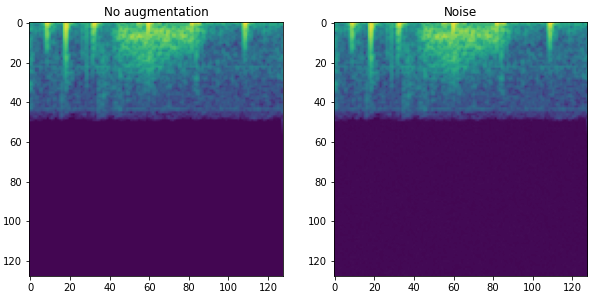
\includegraphics[scale=0.9]{7_0.png}}
		\caption{Noise}
		\label{fig:i7}
	\end{figure}
	\item TimeShift$^{\ref{fig:i8}}$ ~\cite{AudioClassification} \newline Сдвигаем все значения мел-спектрограммы относительно временной оси влево или вправо на |shift|, где $\text{shift} \sim U\{-\text{max\_shift}, \text{max\_shift}\}$, max\_shift - параметр аугментации. Направление сдвига определяется знаком shift: если \newline shift > 0, происходит сдвиг вправо, если shift < 0 - влево. Пустая область, образующаяся в результате сдвига, заполняется нулями.
	\begin{figure}[ht!]
		\center{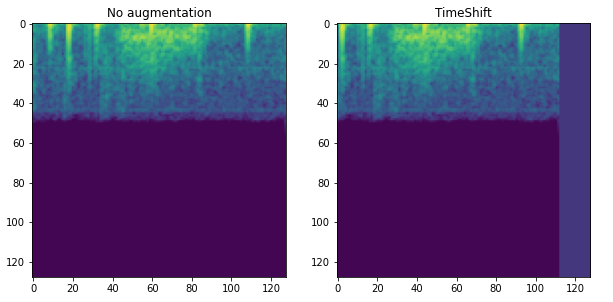
\includegraphics[scale=0.9]{8_0.png}}
		\caption{TimeShift}
		\label{fig:i8}
	\end{figure}
\end{enumerate}

В данной работе мел-спектрограммы нормализуются следующим образом: 

$ value = \frac{value - mean}{std}$, где mean --- математическое ожидание значений мел-спектрограммы, std --- стандартное отклонение. 

Поэтому замена некоторых значений мел-спектрограммы на 0 в результате применения аугментации --- это замена на математическое ожидание.

\section{Предлагаемые подходы}

\subsection{Методы аугментации, основанные на перестановке вертикальных полос в мел-спектрограмме}

Перестановка слов --- метод аугментации, используемый в задачах, связанных с обработкой текстов ~\cite{RandomSwap}. Подобная интуиция может быть применима и к звуковым данным. 

В данной работе предлагается метод \textbf{SwapVerticalStripes}: $^{\ref{fig:i3}}$ \newline
$t \sim U\{0, T\}, t_1 \sim U\{t, \text{TimeSize} - 1 - t\}, t_2 \sim U\{t, \text{TimeSize} - 1 - t\}, |t_1 - t_2| >= t $, \newline $T$ --- параметр аугментации. \newline 
В результате применения аугментации: \newline
$S[0:\text{FreqSize} - 1; t_1: t_1 + t - 1] \leftrightarrow S[0:\text{FreqSize} - 1; t_2 : t_2 + t - 1]$ \newline
Идея метода заключается в перестановке произвольных вертикальных полос в мел-спектрограмме.
\begin{figure}[ht!]
	\center{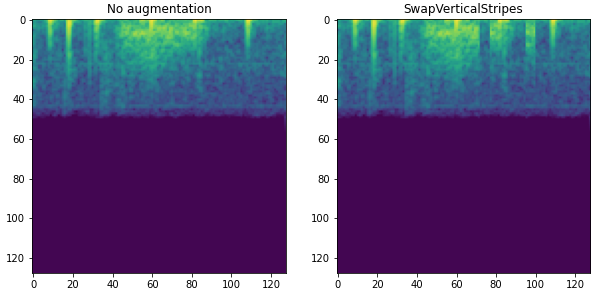
\includegraphics[scale=0.9]{3_0.png}}
	\caption{SwapVerticalStripes}
	\label{fig:i3}
\end{figure}

Также в данной работе предлагаются следующие модификации метода \newline
SwapVerticalStripes:

\begin{enumerate}
    \item \textbf{SwapNeighboringStripes} $^{\ref{fig:i1}}$ \newline
        $t \sim U\{0, T\}, t_0 \sim U\{t, \text{TimeSize} - 1 - t\}$, $T$ --- параметр аугментации. \newline
    	В результате применения аугментации: \newline
    	$S[0:\text{FreqSize} - 1; t_0: t_0 + t - 1] \leftrightarrow S[0:\text{FreqSize} - 1; t_0 - t: t_0 - 1]$ \newline Идея предлагаемого метода SwapNeighboringStripes заключается в перестановке cоседних вертикальных полос.
    	\begin{figure}[ht!]
    	\center{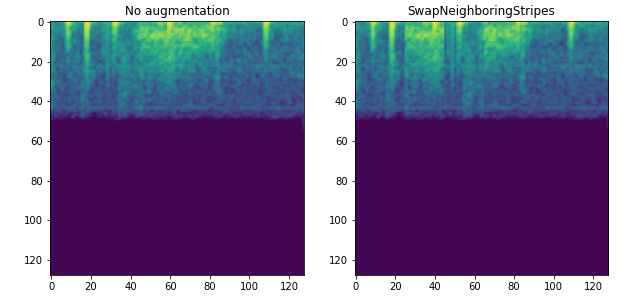
\includegraphics[scale=0.9]{1_0.png}}
    	\caption{SwapNeighboringStripes}
    	\label{fig:i1}
        \end{figure}
    \item \textbf{SwapSeveralStripes} $^{\ref{fig:i2}}$ \newline
        $T, N$ --- параметры аугментации \newline
        $n \sim U\{0, N\}$ \newline
    	В результате применения аугментации (процедура повторяется $n$ раз): \newline
    	$T_0 = \lfloor \frac{T}{n} \rfloor$ \newline
    	$t \sim U\{0, T\}, t_1 \sim U\{t, \text{TimeSize} - 1 - t\}, t_2 \sim U\{t, \text{TimeSize} - 1 - t\}, |t_1 - t_2| >= t $ \newline Идея предлагаемого метода SwapSeveralStripes заключается в перестановке нескольких вертикальных полос.
    	\begin{figure}[ht!]
    	\center{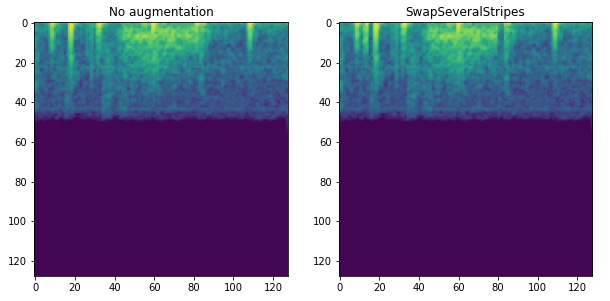
\includegraphics[scale=0.9]{2_0.png}}
    	\caption{SwapSeveralStripes}
    	\label{fig:i2}
        \end{figure}
\end{enumerate}


\subsection{Алгоритм применения методов аугментации с выбором конкретного метода аугментации после каждой эпохи обучения}

Введем следующую операцию: \newline
$\text{Augmentation}(X) = \{\text{Augmentation}(x) \ \forall x \in X\}$, где $X$ --- датасет, \newline $\text{Augmentation}$ --- метод аугментации.

В данной работе предлагается алгоритм \ref{alg:Alg1} применения методов аугментации.

\algrenewcommand\algorithmicdo{\textbf{выполнять}}
\algrenewcommand\algorithmicfor{\textbf{Цикл}}
\algrenewtext{EndFor}{\textbf{Конец цикла}}

\begin{algorithm}
\caption{Предлагаемый алгоритм}\label{alg:Alg1}
\begin{algorithmic}
\State $\text{Augmentations} = \{Augment_1, Augment_2, ..., Augment_n\}$ --- заданный набор аугментаций,
\State $Augment$ --- случайно выбранная аугментация  из $\text{Augmentations}$,
\State $(X_{val}, y_{val})$ --- валидационный датасет, 
\State $(X_{train}, y_{train})$ --- обучающая выборка,
\State $f$ --- метрика качества,
\State $M$ --- число эпох обучения нейронной сети
\For{\textbf{от} $j=1$ \textbf{до} M}
\State train-шаг с применением $Augment$
\State вычисление $F_i = f(Augment_i(X_{val}), y_{val}), i = \overline{1,n}$
\State $Augment = Augment_k$, где $k = argmin_k(F_k)$
\EndFor
\end{algorithmic}
\end{algorithm}

Идея предлагаемого подхода заключается в следующем: в конце n-ой эпохи обучения выбирается метод аугментации, на котором модель нейронной сети работает хуже всего, и далее выбранный метод используется в процессе обучения на n + 1 эпохе.

Стоит отметить, что в работе ~\cite{NearestAlgorithm} подобная идея используется для нахождения "худшего" \ с точки зрения метрика качества на валидационной выборке параметра аугментации, используемого в процессе обучения. 

\newpage
\section{Вычислительные эксперименты}
	
Для исследования применимости предложенных подходов в задаче классификации вычислительные эксперименты проведены с использованием трех датасетов: HeartBeatSounds ~\cite{HeartbeatSoundsArticle}~\cite{HeartbeatSoundsKaggle} (звуки сердцебиения), GTZAN ~\cite{GTZAN_Article}~\cite{GTZAN_kaggle} (классификация музыкальных жанров), Audio MNIST ~\cite{AudioMnistArticle}~\cite{AudioMnistKaggle} (классификация произнесенных человеком цифр).
	
Датасет HeartBeatSounds ~\cite{HeartbeatSoundsArticle}~\cite{HeartbeatSoundsKaggle} представляет собой записи звуков сердцебиения (656 файлов формата .wav). Задача --- определить, к какому из 3 типов относятся звуки на записи: normal, murmur, extrastole.  
	
Датасет GTZAN ~\cite{GTZAN_Article}~\cite{GTZAN_kaggle} состоит из 1000 музыкальных записей (файлов формата .wav). Задача классификации заключается в определении музыкального жанра. Всего в датасете представлено 10 музыкальных жанров: blues, classical, country, disco, hip hop, jazz, metal, pop, reggae, rock.

Датасет Audio MNIST ~\cite{AudioMnistArticle}~\cite{AudioMnistKaggle} состоит из 3000 записей (файлов формата .wav), на которых некоторый человек произносит одну из 10 цифр. Соответственно, задача классификации заключается в том, чтобы определить какую конкретно цифру произносит человек на записи. В данной работе использовалась версия датасета на kaggle ~\cite{AudioMnistKaggle}.

	
В этих датасетах оставлены только корректно считываемые записи, длина которых больше некоторого порогового значения. Из оставшихся файлов в каждом датасете были извлечены фиксированные по длине куски записи (это необходимо для того, чтобы мел-спектрограммы были одного размера), при этом в случае датасета HeartBeatSounds ~\cite{HeartbeatSoundsArticle}~\cite{HeartbeatSoundsKaggle} из одного файла в зависимости от длины записи могло быть извлечено несколько непересекающихся кусков.

Ниже представлено количество элементов в каждом классе в каждом из трех датасетов после предобработки данных:

\begin{itemize}
    \item HeartBeatSounds ~\cite{HeartbeatSoundsArticle}~\cite{HeartbeatSoundsKaggle}
    \begin{enumerate}
        \item normal --- 1296
        \item murmur --- 500
        \item extrastole --- 172
    \end{enumerate}
    \item GTZAN ~\cite{GTZAN_Article}~\cite{GTZAN_kaggle}
    \begin{enumerate}
        \item blues --- 100
        \item classical --- 100
        \item country --- 100
        \item disco --- 100
        \item hip hop --- 100
        \item jazz --- 99
        \item metal --- 100
        \item pop --- 100
        \item reggae --- 100
        \item rock --- 100
    \end{enumerate}
    \item Audio MNIST ~\cite{AudioMnistArticle}~\cite{AudioMnistKaggle}
    \begin{enumerate}
        \item 0 --- 300
        \item 1 --- 289
        \item 2 --- 284
        \item 3 --- 278
        \item 4 --- 294
        \item 5 --- 299
        \item 6 --- 263
        \item 7 --- 300
        \item 8 --- 297
        \item 9 --- 299
    \end{enumerate}
\end{itemize}

В случае датасетов GTZAN ~\cite{GTZAN_Article}~\cite{GTZAN_kaggle} и Audio MNIST ~\cite{AudioMnistArticle}~\cite{AudioMnistKaggle} нет явного дисбаланса классов, поэтому в задачах классификации с этими датасетами использовалась простая в интерпретации метрика качества --- процент верно классифицированных объектов. В случае датасета HeartBeatSounds ~\cite{HeartbeatSoundsArticle}~\cite{HeartbeatSoundsKaggle} присутствует дисбаланс классов, поэтому дополнительно к указанной выше метрике использовалась учитывающая дисбаланс классов метрика качества --- сбалансированная точность. В данной работе использовались модели нейронных сетей resnet18 ~\cite{Resnet}, resnet50 ~\cite{Resnet} и алгоритм оптимизации Adam ~\cite{Adam}. В рамках экспериментов нейронная сеть обучается 100 эпох. Функция потерь --- кросс-энтропия. 
	
В данной работе значения параметров для всех типов аугментаций, где используются эти параметры, считаем равными: 
\begin{itemize}
    \item $F = \lfloor 0.2 \cdot \text{FreqSize} \rfloor$
    \item $T = \lfloor 0.2 \cdot \text{TimeSize} \rfloor$
    \item max\_shift = $\lfloor 0.2 \cdot \text{TimeSize} \rfloor$
    \item $N = 4$
\end{itemize}

Датасеты разбиваются на train\_valid и test в отношении 4 : 1. train\_valid, в свою очередь, разбивается на train и valid в том же отношении. Обучение происходит на выборке train. После обучения берется лучший по метрике результат на валидационной выборке valid и считается метрика на тестовой выборке test. Именно по метрике качества на тестовой выборке оценивается эффективность методов аугментации.
	
Датасеты разбиваются на train, valid и test при 5 разных фиксированных random\_seed. Результаты, соответственно, усредняются. В процессе обучения аугментация применяется с вероятностью $\frac{1}{2}$ к каждому сэмплу в каждом батче.

В качестве методов аугментации для исследования применимости предлагаемого алгоритма был выбран набор из 5 методов: TimeMasking$^{\ref{fig:i5}}$ ~\cite{SpecAugment}, FreqMasking$^{\ref{fig:i6}}$ ~\cite{SpecAugment}, Noise$^{\ref{fig:i7}}$ ~\cite{AudioClassification}, TimeShift$^{\ref{fig:i8}}$ ~\cite{AudioClassification}, SwapVerticalStripes$^{\ref{fig:i3}}$. В рамках экспериментов проводится сравнение предлагаемого алгоритма с RandAugment ~\cite{RandAugment}.

\subsection{Результаты экспериментов}

Результаты экспериментов представлены в таблицах ниже.
\begin{table}[ht!]
    \centering
	\begin{tabular}{| l | l | c |}
    	\hline
	    Метод аугментации & resnet18 & resnet50 \\ \hline
	    Аугментация отсутствует  & 81.98 $\pm$ 2.34 & 82.23 $\pm$ 2.4 \\ \hline
	    SwapVerticalStripes & \textbf{83.2 $\pm$ 1.3} & \textbf{83.65 $\pm$ 1.07} \\ \hline
	    SwapNeighboringStripes & 81.62 $\pm$ 0.69 & \textbf{83.4 $\pm$ 1.71} \\ \hline
	    SwapSeveralStripes & \textbf{83.55 $\pm$ 0.49} & \textbf{84.42 $\pm$ 1.92} \\ \hline
	\end{tabular}
	\caption{Результаты экспериментов (Heartbeat Sounds ~\cite{HeartbeatSoundsArticle}~\cite{HeartbeatSoundsKaggle}) с предлагаемыми методами аугментации SwapVerticalStripes, SwapNeighboringStripes, SwapSeveralStripes. Метрика качества --- процент верно классифицированных объектов.}
	\label{table:lukianov_pavel_t1}
\end{table}

\begin{table}[ht!]
    \centering
	\begin{tabular}{| l | l | c |}
    	\hline
	    Метод аугментации & resnet18 & resnet50 \\ \hline
	    Аугментация отсутствует  & 0.66 $\pm$ 0.034 & 0.692 $\pm$ 0.04 \\ \hline
	    SwapVerticalStripes & \textbf{0.699 $\pm$ 0.029} & 0.681 $\pm$ 0.038 \\ \hline
	    SwapNeighboringStripes & \textbf{0.69 $\pm$ 0.029} & 0.7 $\pm$ 0.027 \\ \hline
	    SwapSeveralStripes & \textbf{0.687 $\pm$ 0.026} & \textbf{0.709 $\pm$ 0.029} \\ \hline
	\end{tabular}
	\caption{Результаты экспериментов (Heartbeat Sounds ~\cite{HeartbeatSoundsArticle}~\cite{HeartbeatSoundsKaggle}) с предлагаемыми методами аугментации SwapVerticalStripes, SwapNeighboringStripes, SwapSeveralStripes. Метрика качества --- сбалансированная точность.}
	\label{table:lukianov_pavel_t1}
\end{table}

\begin{table}[ht!]
    \centering
	\begin{tabular}{| l | l | c |}
    	\hline
	    Метод аугментации & resnet18 & resnet50 \\ \hline
	    Аугментация отсутствует  & 74.3 $\pm$ 3.03 & 73.0 $\pm$ 3.24 \\ \hline
	    SwapVerticalStripes & \textbf{76.6 $\pm$ 2.67} & \textbf{75.6 $\pm$ 3.68} \\ \hline
	    SwapNeighboringStripes & \textbf{75.6 $\pm$ 2.75} & 71.4 $\pm$ 4.91 \\ \hline
	    SwapSeveralStripes & \textbf{75.4 $\pm$ 2.18} & 72.7 $\pm$ 3.4 \\ \hline
	\end{tabular}
	\caption{Результаты экспериментов (GTZAN ~\cite{GTZAN_Article}~\cite{GTZAN_kaggle}) с предлагаемыми методами аугментации SwapVerticalStripes, SwapNeighboringStripes, SwapSeveralStripes. Метрика качества --- процент верно классифицированных объектов.}
	\label{table:lukianov_pavel_t2}
\end{table}

\begin{table}[ht!]
    \centering
	\begin{tabular}{| l | l | c |}
    	\hline
	    Метод аугментации & resnet18 & resnet50 \\ \hline
	    Аугментация отсутствует  & 95.66 $\pm$ 0.81 & 94.49 $\pm$ 0.42 \\ \hline
	    SwapVerticalStripes & 95.42 $\pm$ 0.88 & 95.46 $\pm$  1.05 \\ \hline
	    SwapNeighboringStripes & 95.63 $\pm$ 0.85 & 94.53 $\pm$ 0.4 \\ \hline
	    SwapSeveralStripes & 95.7 $\pm$ 0.52 & 94.39 $\pm$ 0.99 \\ \hline
	\end{tabular}
	\caption{Результаты экспериментов (Audio MNIST ~\cite{AudioMnistArticle}~\cite{AudioMnistKaggle}) с предлагаемыми методами аугментации SwapVerticalStripes, SwapNeighboringStripes, SwapSeveralStripes. Метрика качества --- процент верно классифицированных объектов.}
	\label{table:lukianov_pavel_t2}
\end{table}

\begin{table}[ht!]
    \centering
	\begin{tabular}{| l | l | c |}
    	\hline
	    Метод аугментации & resnet18 & resnet50 \\ \hline
	    Аугментация отсутствует  & 81.98 $\pm$ 2.34 & 82.23 $\pm$ 2.4 \\ \hline
	    RandAugment ~\cite{RandAugment} & 83.1 $\pm$ 0.92 & 84.57 $\pm$ 1.3 \\ \hline
	    Предлагаемый алгоритм & \textbf{86.65 $\pm$ 0.67} & \textbf{86.75 $\pm$ 0.76} \\ \hline
	\end{tabular}
	\caption{Результаты экспериментов (Heartbeat Sounds ~\cite{HeartbeatSoundsArticle}~\cite{HeartbeatSoundsKaggle}) с предлагаемым алгоритмом применения методов аугментации. Метрика качества --- процент верно классифицированных объектов.}
	\label{table:lukianov_pavel_t3}
\end{table}

\begin{table}[ht!]
    \centering
	\begin{tabular}{| l | l | c |}
    	\hline
	    Метод аугментации & resnet18 & resnet50 \\ \hline
	    Аугментация отсутствует  & 0.66 $\pm$ 0.034 & 0.692 $\pm$ 0.04 \\ \hline
	    RandAugment ~\cite{RandAugment} & 0.713 $\pm$ 0.031 & 0.677 $\pm$ 0.036 \\ \hline
	    Предлагаемый алгоритм & \textbf{0.762 $\pm$ 0.023} & \textbf{0.753 $\pm$ 0.02} \\ \hline
	\end{tabular}
	\caption{Результаты экспериментов (Heartbeat Sounds ~\cite{HeartbeatSoundsArticle}~\cite{HeartbeatSoundsKaggle}) с предлагаемым алгоритмом применения методов аугментации. Метрика качества --- сбалансированная точность.}
	\label{table:lukianov_pavel_t3}
\end{table}

\begin{table}[ht!]
    \centering
	\begin{tabular}{| l | l | c |}
    	\hline
	    Метод аугментации & resnet18 & resnet50 \\ \hline
	    Аугментация отсутствует  & 74.3 $\pm$ 3.03 & 73.0 $\pm$ 3.24 \\ \hline
	    RandAugment ~\cite{RandAugment} & 75.0 $\pm$ 2.61 & 74.9 $\pm$ 2.63 \\ \hline
	    Предлагаемый алгоритм & \textbf{76.8 $\pm$ 1.75} & 72.2 $\pm$ 2.8 \\ \hline
	\end{tabular}
	\caption{Результаты экспериментов (GTZAN ~\cite{GTZAN_Article}~\cite{GTZAN_kaggle}) с предлагаемым алгоритмом применения методов аугментации. Метрика качества --- процент верно классифицированных объектов.}
	\label{table:lukianov_pavel_t4}
\end{table}

\begin{table}[ht!]
    \centering
	\begin{tabular}{| l | l | c |}
    	\hline
	    Метод аугментации & resnet18 & resnet50 \\ \hline
	    Аугментация отсутствует  & 95.66 $\pm$ 0.81 & 94.49 $\pm$ 0.42 \\ \hline
	    RandAugment ~\cite{RandAugment} & 95.8 $\pm$ 0.67 & 95.49 $\pm$ 0.77 \\ \hline
	    Предлагаемый алгоритм & 96.04 $\pm$ 0.76 & 94.84 $\pm$ 1.43 \\ \hline
	\end{tabular}
	\caption{Результаты экспериментов (Audio MNIST ~\cite{AudioMnistArticle}~\cite{AudioMnistKaggle}) с предлагаемым алгоритмом применения методов аугментации. Метрика качества --- процент верно классифицированных объектов.}
	\label{table:lukianov_pavel_t3}
\end{table}

\newpage
\subsection{Анализ полученных результатов}

Результаты экспериментов показывают:

\begin{itemize}
    \item В случае датасета Audio MNIST ~\cite{AudioMnistArticle}~\cite{AudioMnistKaggle} с помощью предлагаемых методов SwapVerticalStripes, SwapNeighboringStripes, SwapSeveralStripes и предлагаемого алгоритма применения методов аугментации не удалось получить улучшения в качестве. Стоит отметить, что это может быть связано с особенностью данных или с тем, что и без использования аугментации удается достичь хорошего качества
    \item Использование предлагаемого метода SwapVerticalStripes позволило получить прирост в качестве в задачах аудиоклассификации Heartbeat Sounds Classification
    ~\cite{HeartbeatSoundsArticle}~\cite{HeartbeatSoundsKaggle} (за исключением случая использования resnet50 в качестве нейронной сети и сбалансированной точности в качестве метрики качества) и GTZAN Classification ~\cite{GTZAN_Article}~\cite{GTZAN_kaggle}
    \item Использование предлагаемого метода SwapSeveralStripes позволило получить прирост в качестве в задаче аудиоклассификации Heartbeat Sounds Classification
    ~\cite{HeartbeatSoundsArticle}~\cite{HeartbeatSoundsKaggle}, а также в задаче аудиоклассификации  GTZAN Classification ~\cite{GTZAN_Article}~\cite{GTZAN_kaggle} при использовании resnet18 в качестве нейронной сети
    \item Предлагаемый метод SwapNeighboringStripes показал менее стабильные результаты, чем SwapVerticalStripes и SwapSeveralStripes, однако с его помощью в некоторых случаях можно получить прирост в качестве
    \item В задаче аудиоклассификации Heartbeat Sounds Classification ~\cite{HeartbeatSoundsArticle}~\cite{HeartbeatSoundsKaggle} показано существенное преимущество предлагаемого алгоритма применения методов аугментации над RandAugment ~\cite{RandAugment}
    \item В случае датасета GTZAN ~\cite{GTZAN_Article}~\cite{GTZAN_kaggle} предлагаемый алгоритм позволил получить прирост в качестве относительно RandAugment ~\cite{RandAugment} при использовании модели нейронной сети resnet18, однако в случае resnet50 наблюдается снижение качества не только по сравнению с RandAugment ~\cite{RandAugment}, но и по сравнению с тем случаем, когда обучение нейронной сети происходит без аугментации
\end{itemize}

\section{Заключение}

В процессе выполнения работы получены следующие результаты:

\begin{itemize}
    \item Предложен и реализован метод аугментации аудиоданных SwapVerticalStripes, основанный на перестановке вертикальных полос в мел-спектрограмме, а также его модификации SwapNeighboringStripes, SwapSeveralStripes 
    \item Проведены вычислительные эксперименты, показывающие возможную применимость предложенного метода SwapVerticalStripes и его модификаций в задаче аудиоклассификации
    \item Предложен и реализован алгоритм применения методов аугментации аудиоданных с выбором конкретного метода аугментации после каждой эпохи обучения
    \item Проведены вычислительные, показывающие преимущество предложенного алгоритма над алгоритмом RandAugment ~\cite{RandAugment} в задаче аудиоклассификации Heartbeat Sounds Classification ~\cite{HeartbeatSoundsArticle}~\cite{HeartbeatSoundsKaggle}
\end{itemize}

\begin{thebibliography}{3}
    \addcontentsline{toc}{section}{\bibname}
    \bibitem{Fourier}
    \textit{Harris F.} On the Use of Windows for Harmonic Analysis With the Discrete Fourier Transform // \textit{In Proceedings of the IEEE, Jan. 1978, Vol. 66, Num. 1, 51-83}.
    \bibitem{MelScale}
    \url{https://librosa.org/doc/main/generated/librosa.filters.mel.html}
	\bibitem{RandomErasing}
	\textit{Zhun Zhong, Liang Zheng, Guoliang Kang, Shaozi Li, Yi Yang}. Random Erasing Data Augmentation // \textit{arXiv preprint arXiv:1708.04896.} - 2017.
	\bibitem{RandomErasingClassification}
	\textit{Haiwei Wu, Lin Zhang, Lin Yang, Xuyang Wang, Junjie Wang, Dong Zhang, Ming Li}. Mask Detection and Breath Monitoring from Speech: on Data Augmentation,
	Feature Representation and Modeling // \textit{arXiv preprint arXiv:2008.05175.} - 2020.
	\bibitem{AudioClassification}
	\textit{Steffen Illium, Robert Muller, Andreas Sedlmeier and Claudia Linnhoff-Popien}. Surgical Mask Detection with Convolutional Neural Networks and Data
	Augmentations on Spectrograms // \textit{arXiv preprint arXiv:2008.04590.} - 2020.
	\bibitem{SpecAugment}
	\textit{Daniel S. Park, William Chan, Yu Zhang, Chung-Cheng Chiu, Barret Zoph, Ekin D. Cubuk, Quoc V. Le}. SpecAugment: A Simple Data Augmentation Method
	for Automatic Speech Recognition // \textit{arXiv preprint arXiv:1904.08779.} - 2019.
	\bibitem{SpliceOut}
	\textit{Arjit Jain, Pranay Reddy Samala, Deepak Mittal, Preethi Jyoti, Maneesh Singh}. SpliceOut: A Simple and Efficient Audio Augmentation Method // \textit{arXiv preprint arXiv:2110.00046.} - 2021.
	\bibitem{SpecAugment++}
	\textit{Helin Wang, Yuexian Zou, Wenwu Wang}. SpecAugment++: A Hidden Space Data Augmentation Method for Acoustic Scene Classification // \textit{arXiv preprint arXiv:2103.16858.} - 2021.
	\bibitem{RandAugment}
	\textit{Ekin D. Cubuk, Barret Zoph, Jonathon Shlens, Quoc V. Le}. RandAugment: Practical automated data augmentation with a reduced search space // \textit{arXiv preprint arXiv:1909.13719.} - 2019.
	\bibitem{AutoAugment}
	\textit{Ekin D. Cubuk, Barret Zoph, Dandelion Mane, Vijay Vasudevan, Quoc V. Le}. AutoAugment: Learning Augmentation Policies from Data // \textit{arXiv preprint arXiv:1805.09501.} - 2018.
	\bibitem{MaxUp}
	\textit{Chengyue Gong, Tongzheng Ren, Mao Ye, Qiang Liu}. MaxUp: A Simple Way to Improve Generalization of Neural Network Training // \textit{arXiv preprint arXiv:2002.09024.} - 2020.
	\bibitem{RandomSwap}
	\textit{Jason Wei, Kai Zou}. EDA: Easy Data Augmentation Techniques for Boosting Performance on Text Classification Tasks // \textit{arXiv preprint arXiv:1901.11196.} - 2019.
	\bibitem{NearestAlgorithm}
	\textit{Yu Shen, Laura Zheng, Manli Shu, Weizi Li, Tom Goldstein, Ming C. Lin}. Improving Robustness of Learning-based Autonomous Steering Using Adversarial Images // \textit{arXiv preprint arXiv:2102.13262.} - 2021.
	\bibitem{HeartbeatSoundsArticle}
	\textit{Bentley, P. and Nordehn, G. and Coimbra, M. and Mannor, S.} The {PASCAL} {C}lassifying {H}eart {S}ounds {C}hallenge 2011 {(CHSC2011)} {R}esults. --- 2011.
	\url{http://www.peterjbentley.com/heartchallenge/index.html}
	\bibitem{HeartbeatSoundsKaggle}
	Kaggle-датасет Heartbeat Sounds
	
	\url{https://www.kaggle.com/kinguistics/heartbeat-sounds}
	\bibitem{GTZAN_Article}
    \textit{G. Tzanetakis and P. Cook. Musical genre classification of audio signals.}    // IEEE Transactions on Speech and Audio Processing. --- 2002.
    \bibitem{GTZAN_kaggle}
    GTZAN Dataset --- Music Genre Classification
    
    \url{https://www.kaggle.com/andradaolteanu/gtzan-dataset-music-genre-classification}
    \bibitem{AudioMnistArticle}
    \textit{Sören Becker, Marcel Ackermann, Sebastian Lapuschkin, Klaus-Robert Müller, Wojciech Samek}. Interpreting and Explaining Deep Neural Networks for Classification of Audio Signals // \textit{arXiv preprint arXiv:1807.03418.} --- 2018.
    \bibitem{AudioMnistKaggle}
    Kaggle-датасет Audio MNIST
    
    \url{https://www.kaggle.com/datasets/alanchn31/free-spoken-digits}
    \bibitem{Resnet}
    \textit{Kaiming He, Xiangyu Zhang, Shaoqing Ren, Jian Sun.} Deep Residual Learning for Image Recognition // In Proceedings of the IEEE Conference on Computer Vision and Pattern Recognition (CVPR), 2016, pp. 770-778.
	\bibitem{Adam}
	\textit{Diederik P. Kingma, Jimmy Ba}. Adam: A Method for Stochastic Optimization // In the 3rd International Conference for Learning Representations, San Diego, 2015.
	
\end{thebibliography}

\end{document}
